
\section*{Problema P11.36}

\renewcommand*\thesection{11.36}
\numberwithin{equation}{section}

\begin{center}
    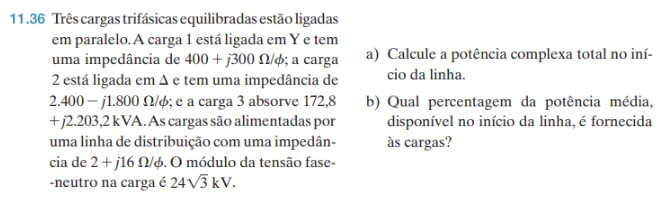
\includegraphics[scale=1.0]{P11.36.jpg}
\end{center}

\subsection*{(a)} 

Começamos identificando a corrente que passa em cada carga, para assim conseguirmos calcular a corrente de fase. Uma vez calculado a corrente
de fase, usamos o fato do circuito estar equilibrado para calcular a corrente total forncecida pela fonte. \\
Na carga 1, que possui impedância $Z_1 = 400 + j300 \un{$\Omega$}$ e está ligada em $Y$, temos

\[ I_1 = \frac{V_a}{Z_1} \logo I_1 = \frac{24000\sqrt{3}\fase{0}}{400 + j300 }  \]

\[ I_1 = 83.14\fase{-36.87} \un{A} = 66.52 - j49.89 \un{A} \]

Na carga 2, ligada em $\Delta$, usamos o mesmo raciocínio da carga 1, mas usando a tensão de linha, uma vez que a 
ligação em $\Delta$ naõ admite conexão ao terminal neutro.

\[ I_2 = \frac{V_{ab}}{Z_2} \logo I_2 = \frac{24000\sqrt{3}\sqrt{3}\fase{0 + 30}}{2400 - j1800}  \]

\[ I_2 = 8\fase{-6.87} \un{A} = 7.94 - j0.96 \un{A} \]

Por fim, para a carga 3, usamos a potência aparente para calcular a corrente, através de  

\[ S_3 = V_a \cdot I_3 \logo I_3 = \left(\frac{S_3}{V_a}\right)^* \]

\[ I_3 = \left(\frac{172800 + j2203200}{24000\sqrt{3}}\right)^* \]

\[ I_3 = 4.15 - j53 \un{A} \]

Com $I_1$, $I_2$ e $I_3$ calculados, temos a corrente total $I_{T_a}$ da fase $a$ dada por   

\[ I_{T_a} = I_1 + I_2 + I_3 \]

\[ I_{T_a} = 78.61 - j103.85 \un{A} \]

Agora calculamos a tensão forncecida pela fonte na fase $a$, considerando a queda causada pela impedância de linha. \\
A queda causada pela linha é  

\[ V_l = Z_l \cdot I_{T_a} \logo V_l =  (2 + j16) \cdot (78.61 - j103.85) \]

\[ V_l = 1818.82 + j1050 \un{V} \]

Assim, a tensão $V_{T_a}$ forncecida pela fase é  

\[ V_{T_a} = V_a + V_l \logo V_{T_a} = 24000\sqrt{3}\fase{0} + 1818.82 + j1050  \]

\[ V_{T_a} = 43.39 + j1.05 \un{kV} \]

Assim, a potência total forncecida pela fase $a$ é  

\[ S_a = V_{T_a} \cdot (I_{T_a})^* \]

\[ S_a = [(43.39 + j1.05)\cdot 10^3] \cdot (78.61 - j103.85)^* \]

\[ S_a = 3.3 + j4.59 \un{MVA} \]

Como o circuito está equilibrado, a potência total forncecida pela fonte (3 fases) é 

\[ S_T = 3 \cdot S_a  \]

\[ \boxed{S_T = 9.9 + j13.77 \un{MVA}} \]


\subsection*{(b)} 

Cada fase apresenta uma queda de tensão indesejada de $V_l = 1818.82 + j1050 \un{V}$ causada pela impedância da linha.
A potência que essa impedância de linha possui é 

\[ S_l = V_l \cdot (I_{T_a})^* \logo S_l = (1818.82 + j1050) \cdot (78.61 - j103.85)^* \]

\[ S_l = 33.93 + j271.42 \un{kVA} \]

Assim, nas 3 fases, a potência total perdida nas impedâncias de linha é  

\[ S_{l_T} = 3 \cdot S_l = 101.79 + j814.26 \un{kVA} \]

Finalmente, o percentual de potência que efetivamente é forncecida às cargas é

\[ S_{\%} = \left|\frac{S_T - S_{l_T}}{S_T}\right|\;100\% \]

\[ S_{\%} = \left|\frac{9.9 + j13.77 - 0.10179 - j0.8142}{9.9 + j13.77}\right|\;100\% \]

\[ S_{\%} = |0.9551 - j0.02315|\;100\% \]

\[ \boxed{S_{\%} = 95.53\%} \]
















